\documentclass[lualatex,ja=standard,a4paper,12pt]{bxjsarticle}
\usepackage{amsmath, amssymb, amsthm}
\usepackage{geometry}
\usepackage{xcolor}
\usepackage{tcolorbox}
\usepackage{booktabs}
\usepackage{array}
\usepackage{graphicx}

\geometry{margin=25mm}

\tcbuselibrary{theorems, skins, breakable}

\newtcolorbox{defbox}[1]{
  colback=blue!5, colframe=blue!60!black,
  fonttitle=\bfseries, title={#1}, arc=3pt, breakable
}
\newtcolorbox{thmbox}[1]{
  colback=green!5, colframe=green!50!black,
  fonttitle=\bfseries, title={#1}, arc=3pt, breakable
}
\newtcolorbox{pointbox}{
  colback=orange!8, colframe=orange!70!black,
  fonttitle=\bfseries, title={ポイント}, arc=3pt, breakable
}
\newtcolorbox{exbox}[1]{
  colback=gray!6, colframe=gray!50,
  fonttitle=\bfseries, title={例：#1}, arc=3pt, breakable
}
\newtcolorbox{warningbox}{
  colback=red!5, colframe=red!60!black,
  fonttitle=\bfseries, title={注意}, arc=3pt, breakable
}

\title{{\large Hoff 第5章} \\[6pt]
       \textbf{5.6\; The Normal Model for Non-Normal Data} \\[4pt]
       {\normalsize （非正規データに対する正規モデル）ゼミ資料}}
\author{}
\date{}

\begin{document}
\maketitle
\thispagestyle{empty}

% ===========================
\section{この節のモチベーション}
% ===========================

正規モデルを使うには「データが正規分布に従う」という仮定が必要なはずである．
しかし実際のデータはしばしば離散・歪み・有界といった非正規な特徴を持つ．
それにもかかわらず，実務では正規モデルが非正規データに広く使われている．

\medskip
なぜそれが正当化できるのか？

\medskip
Hoff の答えはこうである：
個々のデータ点の分布は正規でなくても，
\textbf{標本平均の標本分布は正規分布に近い}（中心極限定理）．
だから「母平均の推論」に限れば正規モデルは有効である．
ただし，それ以外の量（歪度や裾の確率など）の推論には
\textbf{誤った結果}を与えうる——これがこの節の主張である．

\begin{defbox}{準備：標本分布（sampling distribution）とは}
「同じ母集団から同じサイズ $n$ の標本を何度も取り直したら，
統計量（例：標本平均 $\bar{Y}_n$）はどんな値をどんな頻度で取るか」
を表す分布のこと．

\medskip
\textbf{区別が重要：}
\begin{itemize}
  \item \textbf{母集団の分布}：個々のデータ $Y_i$ がどんな値を取るか
  \item \textbf{標本平均の標本分布}：$n$ 個の平均 $\bar{Y}_n$ がどんな値を取るか
\end{itemize}
この節の話はすべて「前者が非正規でも，後者は正規に近づく」という
事実の上に成り立っている．
\end{defbox}

% ===========================
\section{中心極限定理のおさらい}
% ===========================

\begin{thmbox}{中心極限定理（CLT）}
母集団の分布によらず（平均 $\theta$，分散 $\sigma^2$ を持てば），
標本平均 $\bar{Y}_n$ の標本分布は $n$ が大きいほど正規分布に近づく：
\[
  p(\bar{y} \mid \theta, \sigma^2)
  \approx \mathrm{dnorm}\!\left(\bar{y};\; \theta,\, \sqrt{\sigma^2/n}\right).
\]
$n$ が大きくなるにつれて近似の精度は向上する．
\end{thmbox}

\begin{pointbox}
CLT が言っているのは「個々のデータ $y_i$ が正規分布に従う」ではなく，
「\textbf{標本平均 $\bar{y}$ が}近似的に正規分布に従う」ということ．
この違いが，正規モデルが有効な場面（母平均の推論）と
限界（それ以外の推論）を決める．
\end{pointbox}

% ===========================
\section{標本平均の標本分布：Monte Carlo 実験}
% ===========================

\begin{exbox}{GSS データ（子どもの数）}

1998年の General Social Survey（GSS）では，40歳以上の女性921人の
子どもの数が記録されている．この921人を「母集団」とみなし，
そこからサイズ $n$ の無作為標本を取って
母平均（真値は $\theta = 2.42$）を推定する状況を考える．

\medskip
この母集団分布（図の第1パネル）は
\begin{itemize}
  \item \textbf{離散的}（0, 1, 2, \ldots の整数値）
  \item \textbf{有界}（0以上）
  \item \textbf{右に歪んでいる}
\end{itemize}
のに対し，正規分布は連続・非有界・対称なので，正規分布とはほど遠い．

\medskip
\noindent\textbf{モンテカルロ実験：}
$n \in \{5, 15, 45\}$ のそれぞれについて，
921人の母集団から $n$ 人を\textbf{非復元抽出}する操作を
$S$ 回（大きな回数）繰り返し，
得られた $\bar{y}_n^{(1)}, \ldots, \bar{y}_n^{(S)}$ のヒストグラムで
$\bar{Y}_n$ の標本分布を近似する．

\medskip
\noindent\textbf{注：} 実際のGSSの生データが手元にないため，以下の図は
$\mathrm{Poisson}(2.42)$ から生成した $N=921$ の擬似母集団を用いた
モンテカルロシミュレーション（$S=10000$ 回）による再現である．
歪度・分散などの細部は教科書の Figure 5.7 と異なる場合がある．

\begin{center}
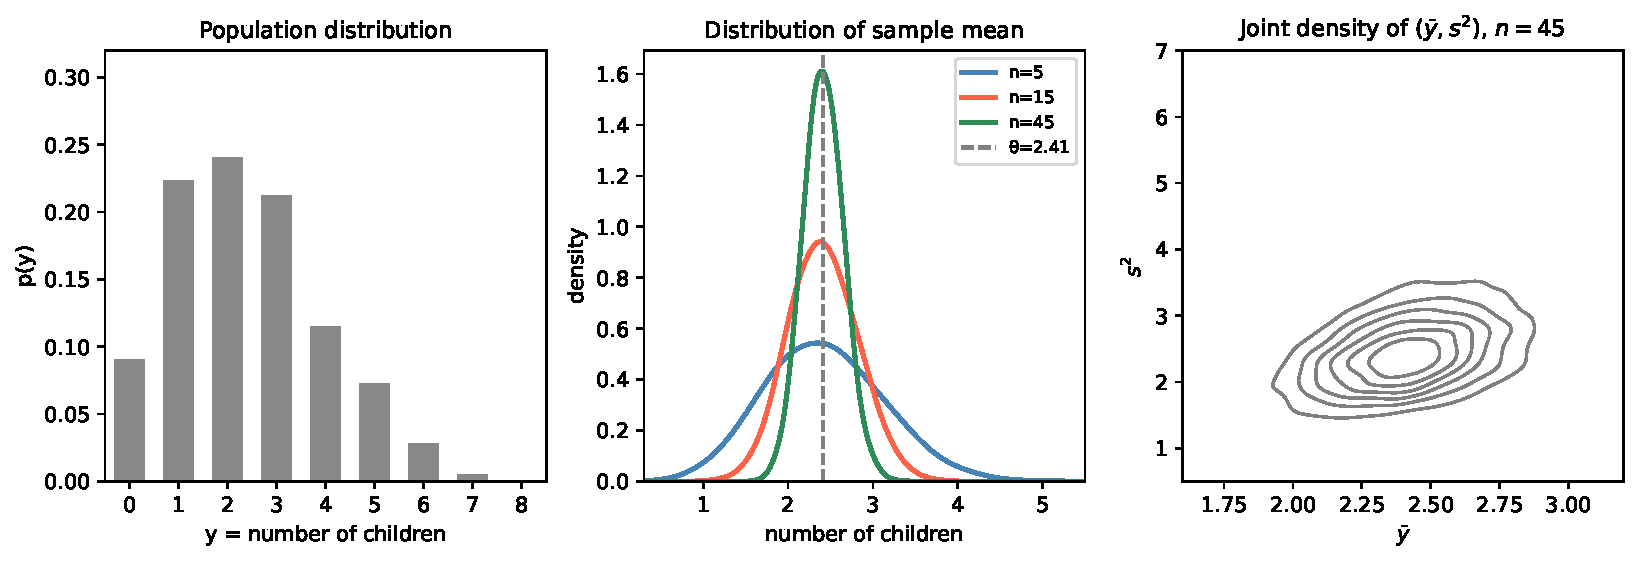
\includegraphics[width=\textwidth]{fig5_7.pdf}
\end{center}

\noindent
\textbf{読み取れること：}
\begin{itemize}
  \item \textbf{第1パネル}：母集団は離散・右歪みで，正規分布とはかけ離れている．
  \item \textbf{第2パネル}：$n=5$ では $\bar{Y}_5$ の分布がやや歪んでいるが，
        $n=15, 45$ では正規分布とほぼ区別がつかない（CLT の効果）．
  \item \textbf{第3パネル}：$n=45$ のときの $\{\bar{Y}, s^2\}$ の同時標本分布．
        $\bar{Y}$ と $s^2$ に\textbf{正の相関}がある（等高線の傾き）．
        右歪みの母集団ではよく見られる現象で，
        「大きい値を引くと平均もばらつきも同時に大きくなる」ため．
        後述のとおり，これが正規モデルの限界に直結する．
\end{itemize}

\end{exbox}

% ===========================
\section{非正規データへの正規モデルの適用}
% ===========================

\subsection*{Step 1：$\sigma^2$ が既知なら話は簡単}

CLT により $p(\bar{y} \mid \theta, \sigma^2)$ は正規密度で近似できるので，
これを尤度として使えば，母平均 $\theta$ の近似事後分布が得られる：
\[
  p(\theta \mid \bar{y}, \sigma^2)
  \;\propto\; p(\theta) \times p(\bar{y} \mid \theta, \sigma^2)
  \;\approx\; p(\theta) \times
    \mathrm{dnorm}\!\left(\bar{y};\; \theta, \sqrt{\sigma^2/n}\right).
\]
ここで注意：使っているデータは生データ $y_1, \ldots, y_n$ ではなく，
その要約である\textbf{標本平均 $\bar{y}$ だけ}である．

\subsection*{Step 2：$\sigma^2$ が未知の場合}

実際には $\sigma^2$ は未知で，標本分散 $s^2$ で推定される．
そこで $(\bar{y}, s^2)$ を条件とした $(\theta, \sigma^2)$ の事後分布を考える：
\begin{align}
  p(\theta, \sigma^2 \mid \bar{y}, s^2)
  &\propto p(\theta, \sigma^2)
    \times p(\bar{y} \mid \theta, \sigma^2)
    \times p(s^2 \mid \bar{y}, \theta, \sigma^2) \notag\\
  &\approx p(\theta, \sigma^2)
    \times \mathrm{dnorm}\!\left(\bar{y};\, \theta, \sqrt{\sigma^2/n}\right)
    \times p(s^2 \mid \bar{y}, \theta, \sigma^2). \tag{5.2}
\end{align}
第2因子（$\bar{y}$ の分布）は CLT で正規近似できる．
問題は\textbf{第3因子 $p(s^2 \mid \bar{y}, \theta, \sigma^2)$ に何を置くか}である．

\subsection*{Step 3：データが本当に正規分布なら}

データが正規母集団からの標本なら，統計理論の古典的な結果
（導出は付録参照）より
\[
  p(s^2 \mid \bar{y}, \theta, \sigma^2)
  = \mathrm{dgamma}\!\left(s^2;\;\frac{n-1}{2},\;\frac{n-1}{2\sigma^2}\right)
\]
が成り立つ．右辺が $\bar{y}$ に依存していないことに注意——
つまり\textbf{正規母集団では $\bar{Y}$ と $s^2$ は独立}である
（実はこれは正規分布を特徴づける性質）．

このガンマ分布を式 (5.2) に代入すると，
生データ $y_1, \ldots, y_n$ をすべて使って計算した通常の事後分布
$p(\theta, \sigma^2 \mid y_1, \ldots, y_n)$ と\textbf{完全に一致する}．
つまり正規データなら「$(\bar{y}, s^2)$ だけを使う」ことによる損失はない．

\subsection*{Step 4：データが非正規なら——同時分布は危険，周辺分布は正確}

しかしデータが非正規なら，$s^2$ はガンマ分布に従うとは限らず，
$\bar{Y}$ とも独立とは限らない．
実際，図の第3パネルで見たとおり GSS 母集団では
$\bar{Y}$ と $s^2$ に正の相関がある．
正規モデルはこの相関を「ゼロ」として扱ってしまうので，
式 (5.2) による $\{\theta, \sigma^2\}$ の\textbf{同時分布の推論は
誤解を招く結果になりうる}．

\medskip
それにもかかわらず，$\theta$ の\textbf{周辺}事後分布は驚くほど正確になりうる．
理由は次の2段階の近似による：
\begin{enumerate}
  \item CLT より，$n$ が大きければ
        $\displaystyle \sqrt{n}\,\frac{\bar{Y} - \theta}{\sigma}
        \;\overset{\cdot}{\sim}\; \mathrm{normal}(0, 1)$
        （$\overset{\cdot}{\sim}$ は「近似的に従う」）．
  \item さらに $n$ が十分大きければ $s^2 \approx \sigma^2$ なので，
        $\sigma$ を $s$ に置き換えても
        \[
          \sqrt{n}\,\frac{\bar{Y} - \theta}{s}
          \;\overset{\cdot}{\sim}\; \mathrm{normal}(0, 1).
        \]
\end{enumerate}
これは入門統計でおなじみの結果と整合する：
正規データなら $\sqrt{n}(\bar{Y} - \theta)/s$ は自由度 $n-1$ の $t$ 分布に従うが，
$n$ が大きいとき $t_{n-1}$ は $\mathrm{normal}(0,1)$ とほぼ同じである．
つまり\textbf{正規モデルから導かれる $\theta$ の推論と，
CLT だけから導かれる $\theta$ の推論が，大標本では一致する}．

\begin{thmbox}{母平均の事後分布（非正規データへの応用）}
$n$ が十分大きければ，データが正規分布に従わなくても，
正規モデルに基づく母平均 $\theta$ の\textbf{周辺}事後分布は
近似的に正しい．
ただし $\{\theta, \sigma^2\}$ の\textbf{同時}事後分布は
（$\bar{Y}$ と $s^2$ の相関が無視されるため）誤解を招く可能性がある．
\end{thmbox}

% ===========================
\section{正規モデルの限界}
% ===========================

\begin{warningbox}
母平均以外の量（歪度，裾の確率，分位点など）については，
正規モデルを非正規データに適用すると\textbf{誤った推論}を与えることがある．

\medskip
理由：正規密度はすべて対称で歪度がゼロだが，
現実の非正規母集団はそうとは限らない．

\medskip
たとえば GSS 母集団の歪度は $E[(Y-\theta)^3]/\sigma^3 = 0.89$（右歪み）
だが，正規モデルはこれを 0 として扱う．
その結果，\textbf{右裾にいる人（子どもが多い人）の割合を過小評価}し，
「子どもの数が多い人の割合」のような推定は不正確になる．
\end{warningbox}

\medskip
\noindent まとめると：

\begin{center}
\renewcommand{\arraystretch}{1.6}
\begin{tabular}{lcc}
\toprule
推論対象 & 正規モデルの適用 & 理由 \\
\midrule
母平均 $\theta$（周辺） & 有効（大標本） & CLT により $\bar{y}$ が正規近似できる \\
$(\theta, \sigma^2)$ の同時分布 & 注意が必要 & $\bar{y}$ と $s^2$ の相関が無視される \\
歪度・裾の確率・分位点 & 不適切 & 正規分布は常に対称・歪度ゼロ \\
\bottomrule
\end{tabular}
\end{center}

% ===========================
\section{まとめ}
% ===========================

\begin{thmbox}{5.6節のまとめ}
\begin{enumerate}
  \item 非正規データに正規モデルを使う根拠は
        「データが正規分布に従う」ことではなく，
        「\textbf{標本平均が正規分布で近似できる}」という CLT にある．

  \item モンテカルロ実験（GSS データ）により，非正規母集団でも
        $n$ が増えるにつれて $\bar{Y}_n$ の標本分布が
        正規分布に近づくことが確認できる．

  \item 正規データなら $\bar{Y}$ と $s^2$ は独立で，
        $(\bar{y}, s^2)$ に基づく事後分布は生データに基づく事後分布と一致する．
        非正規データではこの独立性が崩れる
        （GSS の例では正の相関）ため，
        $\{\theta, \sigma^2\}$ の\textbf{同時}推論は誤解を招きうる．

  \item それでも，母平均 $\theta$ の\textbf{周辺}事後分布は
        大標本で近似的に正しい
        （$\sqrt{n}(\bar{Y}-\theta)/s \overset{\cdot}{\sim} \mathrm{normal}(0,1)$
        が母集団の形によらず成り立つため）．

  \item ただし正規モデルが有効なのは\textbf{母平均の推論に限られる}．
        歪度や裾の確率など分布の形に関わる量には不適切であり，
        そのような量の推論には非正規モデルが必要になる．
\end{enumerate}
\end{thmbox}

\appendix
% ===========================
\section{付録：正規データにおける $s^2$ のガンマ分布と
$\bar{Y}$，$s^2$ の独立性}
% ===========================

本編 Step 3 で使った次の結果について，その意味を詳しく確認する．

\begin{thmbox}{正規母集団における $s^2$ の標本分布}
データ $Y_1, \ldots, Y_n$ が本当に $\mathrm{Normal}(\theta, \sigma^2)$
からの i.i.d. 標本ならば，
\[
  p(s^2 \mid \bar{y}, \theta, \sigma^2)
  = \mathrm{dgamma}\!\left(s^2;\;\frac{n-1}{2},\;\frac{n-1}{2\sigma^2}\right).
\]
\end{thmbox}

\subsection{どこから来た式か：カイ二乗分布の言い換え}

これは入門統計でおなじみの結果
\[
  \frac{(n-1)\,s^2}{\sigma^2} \;\sim\; \chi^2_{n-1}
\]
をガンマ分布の言葉で書き直したものである．
カイ二乗分布はガンマ分布の特殊ケースで，
$\chi^2_{\nu} = \mathrm{Gamma}(\nu/2,\, 1/2)$ が成り立つ．
$X \sim \mathrm{Gamma}(a, b)$ のとき $cX \sim \mathrm{Gamma}(a, b/c)$
という尺度変換の性質を使うと，
\[
  \frac{(n-1)s^2}{\sigma^2} \sim \mathrm{Gamma}\!\left(\frac{n-1}{2}, \frac{1}{2}\right)
  \;\Longrightarrow\;
  s^2 \sim \mathrm{Gamma}\!\left(\frac{n-1}{2}, \frac{n-1}{2\sigma^2}\right)
\]
となり，本文の式が得られる．

\subsection{なぜ $(n-1)s^2/\sigma^2 \sim \chi^2_{n-1}$ なのか：導出}

前小節で「おなじみの結果」として使った
$(n-1)s^2/\sigma^2 \sim \chi^2_{n-1}$ を，
線形代数の言葉で導出する．
この導出は同時に「$\bar{Y}$ と $s^2$ の独立性」も証明してしまう．

\begin{defbox}{カイ二乗分布の定義}
$Z_1, \ldots, Z_\nu$ が i.i.d. $\mathrm{Normal}(0,1)$ のとき，
\[
  Z_1^2 + Z_2^2 + \cdots + Z_\nu^2 \;\sim\; \chi^2_\nu
\]
と定義する．$\nu$ を\textbf{自由度}と呼ぶ．
つまり $\chi^2_\nu$ とは「独立な標準正規変数 $\nu$ 個の2乗和の分布」のこと．
\end{defbox}

\subsubsection*{Step 1：標準化と平方和の分解}

$Y_i \sim \mathrm{Normal}(\theta, \sigma^2)$ を標準化して
$Z_i = (Y_i - \theta)/\sigma \sim \mathrm{Normal}(0,1)$（i.i.d.）とする．
恒等式
\[
  \sum_{i=1}^n (Y_i - \theta)^2
  = \sum_{i=1}^n (Y_i - \bar{Y})^2 + n(\bar{Y} - \theta)^2
\]
（$\pm\bar{Y}$ を挟んで展開すると交差項が消える）の両辺を
$\sigma^2$ で割ると
\[
  \underbrace{\sum_{i=1}^n Z_i^2}_{\chi^2_n}
  = \underbrace{\frac{(n-1)s^2}{\sigma^2}}_{?}
  + \underbrace{\left(\sqrt{n}\,\frac{\bar{Y}-\theta}{\sigma}\right)^2}_{\chi^2_1}.
\]
左辺は定義から $\chi^2_n$，右辺第2項は標準正規変数1個の2乗なので $\chi^2_1$．
すると「残りの第1項は $\chi^2_{n-1}$ になるはず」と予想できるが，
右辺の2つの項が独立かどうか分からないので，このままでは証明にならない．
きちんと示すには次の Step 2 が必要である．

\subsubsection*{Step 2：直交変換（回転）を使う}

鍵になるのは標準正規ベクトルの\textbf{回転不変性}：

\begin{thmbox}{標準正規ベクトルの回転不変性}
$\boldsymbol{Z} = (Z_1, \ldots, Z_n)^\top$ の成分が i.i.d.
$\mathrm{Normal}(0,1)$ で，$Q$ が $n \times n$ 直交行列
（$Q^\top Q = I$）ならば，
$\boldsymbol{W} = Q\boldsymbol{Z}$ の成分も i.i.d. $\mathrm{Normal}(0,1)$．
\end{thmbox}

\paragraph{証明}
まず，密度の変数変換の公式を確認する．
確率密度は「確率 $\div$ 体積」なので，
変換が空間の体積を伸縮させる場合は密度に補正が必要になる．
1次元の例：$W = 2Z$ とすると，区間 $[0, 0.1]$ にあった $Z$ の確率は
そっくり区間 $[0, 0.2]$ の $W$ に移る．同じ確率が2倍の長さに
薄く延ばされるので，$W$ の密度は対応する点の $Z$ の密度の $1/2$ になる．
この「2倍」を測るのが\textbf{ヤコビアン}である．
一般に可逆な線形変換 $\boldsymbol{W} = Q\boldsymbol{Z}$ に対して
\[
  p_W(\boldsymbol{w})
  = p_Z(Q^{-1}\boldsymbol{w}) \cdot
    \left|\det \frac{\partial \boldsymbol{z}}{\partial \boldsymbol{w}}\right|
  = p_Z(Q^{-1}\boldsymbol{w}) \cdot |\det Q^{-1}|
\]
が成り立つ（$|\det|$ は線形写像が単位体積を何倍にするかを表す量で，
これで「確率 $\div$ 体積」の帳尻が合う）．

\medskip
$Q$ が\textbf{直交行列}の場合，これは回転（または鏡映）であり，
空間を回すだけで伸び縮みさせない．実際，$Q^\top Q = I$ より
\[
  (\det Q)^2 = \det(Q^\top Q) = \det I = 1
  \quad\Longrightarrow\quad
  |\det Q| = |\det Q^{-1}| = 1
\]
なので体積補正は不要で，$Q^{-1} = Q^\top$ にも注意すると
\[
  p_W(\boldsymbol{w}) = p_Z(Q^\top \boldsymbol{w}).
\]

\medskip
次に，$\boldsymbol{Z}$ の密度が\textbf{ノルムのみに依存する}ことを使う：
\[
  p_Z(\boldsymbol{z})
  = \prod_{i=1}^n \frac{1}{\sqrt{2\pi}} e^{-z_i^2/2}
  = (2\pi)^{-n/2}\, e^{-\|\boldsymbol{z}\|^2/2}.
\]
直交変換はノルムを保つ（$\|Q^\top\boldsymbol{w}\|^2
= \boldsymbol{w}^\top Q Q^\top \boldsymbol{w} = \|\boldsymbol{w}\|^2$）ので，
\[
  p_W(\boldsymbol{w})
  = (2\pi)^{-n/2}\, e^{-\|Q^\top\boldsymbol{w}\|^2/2}
  = (2\pi)^{-n/2}\, e^{-\|\boldsymbol{w}\|^2/2}.
\]
これは $\boldsymbol{Z}$ の密度と全く同じ形，
すなわち $\boldsymbol{W}$ の成分も i.i.d. $\mathrm{Normal}(0,1)$ である．
\hfill $\blacksquare$

\begin{pointbox}
証明は2つの事実の組み合わせである：
\textbf{(i) ヤコビアンが1}（回転は体積を保つので密度に余計な係数がつかない），
\textbf{(ii) 密度がノルムだけの関数}（回転はノルムを保つので密度の値も変わらない）．
もし $Q$ が直交でない行列（たとえば拡大）だったら，
(i) の段階で $1/|\det Q|$ が残ってしまい，標準正規にはならない．
\end{pointbox}

\medskip
そこで，\textbf{第1行が}
$\boldsymbol{q}_1 = \left(\tfrac{1}{\sqrt{n}}, \tfrac{1}{\sqrt{n}}, \ldots, \tfrac{1}{\sqrt{n}}\right)$
であるような直交行列 $Q$ を1つ取る．

\paragraph{なぜ第1行をこう選ぶのか}
狙いは「標本平均を1つの座標に押し込める」ことである．
$\boldsymbol{W} = Q\boldsymbol{Z}$ の第1成分は
第1行と $\boldsymbol{Z}$ の内積なので，
\[
  W_1 = \boldsymbol{q}_1 \cdot \boldsymbol{Z}
      = \frac{1}{\sqrt{n}}\sum_{i=1}^n Z_i = \sqrt{n}\,\bar{Z}
\]
となり，標本平均の情報が $W_1$ \textbf{だけ}に集約される．
係数を $1/n$ でなく $1/\sqrt{n}$ にしているのは，
第1行の長さを1にするため
（$\|\boldsymbol{q}_1\|^2 = n \cdot \frac{1}{n} = 1$）である．
直交行列の行はすべて長さ1でなければならない．

\paragraph{なぜそのような $Q$ が必ず存在するのか}
直交行列とは「各行が長さ1で，互いに直交する」行列，
言い換えれば\textbf{行たちが $\mathbb{R}^n$ の正規直交基底をなす}行列である．
問題は「$\boldsymbol{q}_1$ を第1ベクトルとする正規直交基底が作れるか」だが，
これは線形代数の標準的な手続きでできる：
\begin{enumerate}
  \item $\boldsymbol{q}_1$ に適当なベクトル（たとえば標準基底
        $\boldsymbol{e}_1, \ldots, \boldsymbol{e}_n$ のうち $n-1$ 本）を
        追加して $\mathbb{R}^n$ の基底を作る．
  \item この基底に\textbf{グラム・シュミットの直交化}を施す．
        先頭の $\boldsymbol{q}_1$ はすでに長さ1なのでそのまま残り，
        続くベクトルは順に「それまでのベクトルとの直交成分を取り出して
        正規化」される．
\end{enumerate}
結果として $\boldsymbol{q}_1$ を第1行に持つ正規直交基底
$\{\boldsymbol{q}_1, \boldsymbol{q}_2, \ldots, \boldsymbol{q}_n\}$ が得られ，
これを並べれば所望の直交行列 $Q$ になる．
なお $Q$ の選び方は一意ではないが，
証明には「1つ存在する」ことさえ分かれば十分である
（どの $Q$ を選んでも $W_1$ と $\sum_{i \geq 2} W_i^2$ は同じ）．

\paragraph{具体例：Helmert 行列}
明示的な構成としては \textbf{Helmert 行列}が知られている．
第 $k$ 行（$k = 2, \ldots, n$）を
「最初の $k-1$ 成分が $1$，第 $k$ 成分が $-(k-1)$，残りは $0$，
全体を $\sqrt{k(k-1)}$ で割ったもの」とする．
$n = 3$ の場合：
\[
  Q =
  \begin{pmatrix}
    \frac{1}{\sqrt{3}} & \frac{1}{\sqrt{3}} & \frac{1}{\sqrt{3}} \\[4pt]
    \frac{1}{\sqrt{2}} & -\frac{1}{\sqrt{2}} & 0 \\[4pt]
    \frac{1}{\sqrt{6}} & \frac{1}{\sqrt{6}} & -\frac{2}{\sqrt{6}}
  \end{pmatrix}.
\]
各行の長さが1であること，どの2行も内積が0であることは
直接計算で確認できる（たとえば第1行と第2行：
$\frac{1}{\sqrt{6}} - \frac{1}{\sqrt{6}} + 0 = 0$）．
第2行以降はどれも「成分の和が0」，
つまり $\boldsymbol{1} = (1, \ldots, 1)$ と直交する方向を向いている——
これが後で述べる「偏差ベクトルの住む $n-1$ 次元部分空間」の
正規直交基底になっている．

\medskip
以上の $Q$ を使って $\boldsymbol{W} = Q\boldsymbol{Z}$ とおくと：

\begin{itemize}
  \item \textbf{第1成分}：
        $\displaystyle W_1 = \frac{1}{\sqrt{n}}\sum_{i=1}^n Z_i = \sqrt{n}\,\bar{Z}$．
  \item \textbf{ノルムの保存}：直交変換は長さを変えないので
        $\displaystyle \sum_{i=1}^n W_i^2 = \sum_{i=1}^n Z_i^2$．
\end{itemize}

したがって，
\[
  \sum_{i=2}^n W_i^2
  = \sum_{i=1}^n Z_i^2 - W_1^2
  = \sum_{i=1}^n Z_i^2 - n\bar{Z}^2
  = \sum_{i=1}^n (Z_i - \bar{Z})^2
  = \frac{(n-1)s^2}{\sigma^2}.
\]

\subsubsection*{Step 3：結論——分布と独立性が同時に出る}

回転不変性より $W_1, W_2, \ldots, W_n$ は i.i.d. $\mathrm{Normal}(0,1)$．よって：

\begin{enumerate}
  \item $\displaystyle \frac{(n-1)s^2}{\sigma^2} = \sum_{i=2}^n W_i^2$ は
        独立な標準正規変数 \textbf{$n-1$ 個}の2乗和なので，
        定義により $\chi^2_{n-1}$ に従う．
  \item $\bar{Y}$ は $W_1$ だけの関数（$\bar{Y} = \theta + \sigma W_1/\sqrt{n}$），
        $s^2$ は $W_2, \ldots, W_n$ だけの関数．
        $W_1$ と $(W_2, \ldots, W_n)$ は独立なので，
        \textbf{$\bar{Y}$ と $s^2$ は独立}．
\end{enumerate}

\begin{pointbox}
\textbf{自由度 $n-1$ の正体：}
偏差ベクトル $(Y_1 - \bar{Y}, \ldots, Y_n - \bar{Y})$ は
制約 $\sum_i (Y_i - \bar{Y}) = 0$ を満たすので，
$n$ 次元空間の中の $n-1$ 次元部分空間（$\boldsymbol{1}$ の直交補空間）
に住んでいる．
上の直交変換はこの部分空間の正規直交基底 $(W_2, \ldots, W_n)$ を
取り出す操作であり，「自由に動ける方向が $n-1$ 個」だから自由度 $n-1$．

\medskip
また，この導出のどこで\textbf{正規性}を使ったかに注意：
回転不変性（密度が $\|\boldsymbol{z}\|$ のみに依存すること）は
正規分布の性質である．
非正規データではこの議論が使えず，
実際に $\bar{Y}$ と $s^2$ の独立性もガンマ分布性も崩れる——
これが本編 Step 4 の話につながる．
\end{pointbox}

\subsection{「右辺に $\bar{y}$ がない」ことの意味：独立性}

左辺 $p(s^2 \mid \bar{y}, \theta, \sigma^2)$ は
「$\bar{y}$ を\textbf{与えたときの}」$s^2$ の条件付き分布なのに，
右辺のガンマ密度には $\bar{y}$ が一切登場しない．
条件に入れても分布が変わらない——これはまさに
\[
  \text{正規母集団では } \bar{Y} \text{ と } s^2 \text{ は\textbf{独立}}
\]
ということである．

\begin{pointbox}
直感的には：正規母集団では
「標本の平均が\textbf{どこ}にあるか（$\bar{Y}$）」と
「標本が\textbf{どれくらい散らばって}いるか（$s^2$）」
が互いに無関係，ということ．

\medskip
実はこの独立性は\textbf{正規分布だけが持つ}特徴的な性質である
（Lukacs (1942)；5.7節で言及される）．
つまり「$\bar{Y}$ と $s^2$ が独立」なら母集団は正規分布しかありえない．
\end{pointbox}

\subsection{代入すると生データの事後分布と完全に一致する}

このガンマ分布を式 (5.2) の第3因子に代入して得られる
$(\theta, \sigma^2)$ の事後分布は，
生データ $y_1, \ldots, y_n$ をすべて使って計算した通常の事後分布
$p(\theta, \sigma^2 \mid y_1, \ldots, y_n)$（5.3節の結果）と
\textbf{厳密に一致する}．これを証明する．

\paragraph{証明の方針}
2つの事後分布はどちらも
\[
  \text{事後分布} \;\propto\; \text{事前分布 } p(\theta, \sigma^2)
  \;\times\; \text{尤度}
\]
の形をしている．事前分布は共通なので，
\textbf{2つの尤度が $(\theta, \sigma^2)$ の関数として比例する}
ことを示せばよい
（比例定数がデータのみに依存し $(\theta,\sigma^2)$ を含まなければ，
正規化した後の事後分布は完全に同じになる）．

\paragraph{尤度1：生データの尤度}
$Y_i \sim$ i.i.d. $\mathrm{Normal}(\theta, \sigma^2)$ の同時密度は
\[
  p(y_1, \ldots, y_n \mid \theta, \sigma^2)
  = \prod_{i=1}^n \frac{1}{\sqrt{2\pi\sigma^2}}
    \exp\!\left\{-\frac{(y_i - \theta)^2}{2\sigma^2}\right\}
  = (2\pi\sigma^2)^{-n/2}
    \exp\!\left\{-\frac{\sum_i (y_i - \theta)^2}{2\sigma^2}\right\}.
\]
ここで A.2 節の Step 1 でも使った平方和の分解
\[
  \sum_{i=1}^n (y_i - \theta)^2 = (n-1)s^2 + n(\bar{y} - \theta)^2
\]
を代入すると
\[
  p(y_1, \ldots, y_n \mid \theta, \sigma^2)
  = (2\pi)^{-n/2} \,(\sigma^2)^{-n/2}
    \exp\!\left\{-\frac{(n-1)s^2 + n(\bar{y} - \theta)^2}{2\sigma^2}\right\}.
\]
この時点で，尤度がデータに $(\bar{y}, s^2)$ を通じてしか
依存しないことが見て取れる（十分性）．

\paragraph{尤度2：$(\bar{y}, s^2)$ の尤度}
一方，式 (5.2) の第2・第3因子は，
A.3 節で示した $\bar{Y}$ と $s^2$ の独立性を使うと
$(\bar{y}, s^2)$ の同時密度そのものであり，
\[
  p(\bar{y}, s^2 \mid \theta, \sigma^2)
  = \underbrace{\sqrt{\frac{n}{2\pi\sigma^2}}
    \exp\!\left\{-\frac{n(\bar{y}-\theta)^2}{2\sigma^2}\right\}}_{
      \mathrm{dnorm}(\bar{y};\,\theta,\sqrt{\sigma^2/n})}
  \;\times\;
  \underbrace{\frac{\left(\frac{n-1}{2\sigma^2}\right)^{\frac{n-1}{2}}}{\Gamma\!\left(\frac{n-1}{2}\right)}
    (s^2)^{\frac{n-1}{2}-1}
    \exp\!\left\{-\frac{(n-1)s^2}{2\sigma^2}\right\}}_{
      \mathrm{dgamma}\left(s^2;\,\frac{n-1}{2},\,\frac{n-1}{2\sigma^2}\right)}.
\]
これを $(\theta, \sigma^2)$ の関数として整理する．
$(\theta, \sigma^2)$ を含まない因子
（$\sqrt{n/2\pi}$，$\Gamma(\cdot)$，$(n-1)^{(n-1)/2}$，$(s^2)^{\cdots}$ など）
をすべて比例定数に押し込むと，
$\sigma^2$ の冪は $(\sigma^2)^{-1/2} \times (\sigma^2)^{-(n-1)/2}
= (\sigma^2)^{-n/2}$ となり，
\[
  p(\bar{y}, s^2 \mid \theta, \sigma^2)
  \;\propto\;
  (\sigma^2)^{-n/2}
    \exp\!\left\{-\frac{(n-1)s^2 + n(\bar{y} - \theta)^2}{2\sigma^2}\right\}.
\]

\paragraph{比較}
尤度1と尤度2は，$(\theta, \sigma^2)$ の関数として
\textbf{全く同じ形} $(\sigma^2)^{-n/2}
\exp\{-[(n-1)s^2 + n(\bar{y}-\theta)^2]/(2\sigma^2)\}$
に比例している．したがって
\[
  p(\theta, \sigma^2 \mid y_1, \ldots, y_n)
  \;\propto\; p(\theta, \sigma^2) \times p(y_1, \ldots, y_n \mid \theta, \sigma^2)
  \;\propto\; p(\theta, \sigma^2) \times p(\bar{y}, s^2 \mid \theta, \sigma^2)
  \;\propto\; p(\theta, \sigma^2 \mid \bar{y}, s^2)
\]
であり，両辺とも積分すると1になる確率分布なので，
比例ではなく\textbf{等しい}：
\[
  p(\theta, \sigma^2 \mid y_1, \ldots, y_n)
  = p(\theta, \sigma^2 \mid \bar{y}, s^2).
  \qquad \blacksquare
\]

\begin{pointbox}
証明の核心は，平方和の分解によって生データの尤度が
\[
  (\sigma^2)^{-n/2}
  \exp\!\left\{-\frac{(n-1)s^2 + n(\bar{y}-\theta)^2}{2\sigma^2}\right\}
\]
という「$(\bar{y}, s^2)$ だけで書ける形」になることである．
$\sigma^2$ の冪の勘定では，
正規密度から $-1/2$，ガンマ密度から $-(n-1)/2$ が出て
合計 $-n/2$ となり，生データ尤度の $(\sigma^2)^{-n/2}$ と
ちょうど一致する——$n$ 個分の情報が
「平均に1個分＋分散に $n-1$ 個分」と配分されている，と読める．
\end{pointbox}

\medskip
つまり正規モデルでは，
$n$ 個のデータを $(\bar{y}, s^2)$ の\textbf{2つの数字に要約しても
情報は何も失われない}．
これは $(\bar{y}, s^2)$ が正規モデルの\textbf{十分統計量}である
ことの現れである（3.3節・5.5節参照）．

\subsection{この結果が5.6節で果たす役割}

この付録の内容は，非正規データの議論のための「基準点」である．
論理の流れを整理すると：

\begin{enumerate}
  \item \textbf{正規データなら}：$s^2$ はガンマ分布に従い，$\bar{Y}$ と独立．
        $(\bar{y}, s^2)$ ベースの事後分布は生データベースの事後分布と
        完全一致（＝何も問題ない）．
  \item \textbf{非正規データなら}：$s^2$ はガンマ分布に従うとは限らず，
        $\bar{Y}$ と独立とも限らない．
        実際 GSS 母集団では正の相関がある（図の第3パネル）．
        正規モデルはこの相関をゼロと扱うので，
        $(\theta, \sigma^2)$ の\textbf{同時}推論は誤解を招きうる．
  \item \textbf{それでも}：$\theta$ の\textbf{周辺}事後分布は
        CLT により大標本で近似的に正しい（本編 Step 4）．
\end{enumerate}

正規データの場合（1）が「完璧」であるだけに，
非正規データで何が崩れるのか（2）が明確になる——
崩れるのは\textbf{ガンマ分布性と独立性}であり，
それが同時推論の信頼性を損なう，という構造である．

% ===========================
\section{付録：大標本近似の詳細——$s^2 \approx \sigma^2$ と
$t_{n-1} \approx \mathrm{normal}(0,1)$}
% ===========================

本編 Step 4 では次の2つの近似を使った：
\begin{enumerate}
  \item $n$ が十分大きければ $s^2 \approx \sigma^2$
  \item $n$ が大きければ $t_{n-1}$ 分布は $\mathrm{normal}(0,1)$ とほぼ同じ
\end{enumerate}
この付録ではそれぞれの理由を説明し，
教科書の ``This should seem familiar'' の一節
（正規データなら $\sqrt{n}(\bar{Y}-\theta)/s \sim t_{n-1}$）が
付録 A の結果から導けることも確認する．

\subsection{なぜ $s^2 \approx \sigma^2$ なのか：大数の法則}

\begin{thmbox}{大数の法則（LLN）}
$X_1, X_2, \ldots$ が i.i.d. で $E[X_i]$ が有限ならば，
$n \to \infty$ のとき
\[
  \frac{1}{n}\sum_{i=1}^n X_i \;\longrightarrow\; E[X_1].
\]
「i.i.d. な量の平均は，$n$ が大きくなるとその期待値に収束する」．
\end{thmbox}

$\bar{Y} \to \theta$ はこの定理を $X_i = Y_i$ に適用したものだが，
同じ定理を\textbf{2乗 $X_i = Y_i^2$ にも}適用できる：
$\frac{1}{n}\sum Y_i^2 \to E[Y^2]$．
標本分散を
\[
  s^2 = \frac{1}{n-1}\sum_{i=1}^n (Y_i - \bar{Y})^2
      = \frac{n}{n-1}\left[\frac{1}{n}\sum_{i=1}^n Y_i^2 - \bar{Y}^2\right]
\]
と変形すると（展開して整理すればよい），$n \to \infty$ で
\begin{itemize}
  \item $\frac{1}{n}\sum Y_i^2 \;\to\; E[Y^2]$（LLN），
  \item $\bar{Y}^2 \;\to\; \theta^2$（LLN），
  \item $\frac{n}{n-1} \;\to\; 1$
\end{itemize}
なので
\[
  s^2 \;\longrightarrow\; E[Y^2] - \theta^2 = \mathrm{Var}[Y] = \sigma^2.
\]
最後の等号は分散の定義
$\mathrm{Var}[Y] = E[Y^2] - (E[Y])^2$ そのものである．

\medskip
\noindent 別の見方をすると：
\begin{itemize}
  \item \textbf{中心は正しい}：$E[s^2] = \sigma^2$
        （$n-1$ で割る不偏分散は，どんな $n$ でも期待値がぴったり $\sigma^2$）
  \item \textbf{ばらつきは消える}：$\mathrm{Var}[s^2]$ は
        $O(1/n)$ で $0$ に向かう（4次モーメントが有限なら）
\end{itemize}
「期待値が $\sigma^2$ で，その周りのばらつきが潰れていく」ので
$s^2$ は $\sigma^2$ の近くに集中する
（$s^2$ は $\sigma^2$ の\textbf{一致推定量}である）．

\begin{pointbox}
この収束に\textbf{正規性は一切不要}である
（必要なのは該当モーメントの有限性だけ）．
だからこそ非正規データでも，CLT（これも正規性不要）と組み合わせて
\[
  \sqrt{n}\,\frac{\bar{Y} - \theta}{\sigma}
  \;\overset{\cdot}{\sim}\; \mathrm{normal}(0,1)
  \quad\xrightarrow{\;s^2 \approx \sigma^2\;}\quad
  \sqrt{n}\,\frac{\bar{Y} - \theta}{s}
  \;\overset{\cdot}{\sim}\; \mathrm{normal}(0,1)
\]
が母集団の形によらず成り立つ．
なお「分母を $\sigma$ から $s$ に差し替えても分布収束が壊れない」
ことを厳密に保証する道具は \textbf{Slutsky の定理}と呼ばれる．
\end{pointbox}

\subsection{正規データなら $\sqrt{n}(\bar{Y}-\theta)/s \sim t_{n-1}$：
付録 A からの導出}

教科書が ``Recall from introductory statistics'' として引く
この事実は，実は付録 A で示した2つの結果から直ちに従う．

\begin{defbox}{$t$ 分布の定義}
$Z \sim \mathrm{Normal}(0,1)$ と $V \sim \chi^2_\nu$ が\textbf{独立}のとき，
\[
  T = \frac{Z}{\sqrt{V/\nu}} \;\sim\; t_\nu
\]
と定義する（自由度 $\nu$ の $t$ 分布）．
\end{defbox}

正規データに対して，
\[
  Z = \sqrt{n}\,\frac{\bar{Y}-\theta}{\sigma} \sim \mathrm{Normal}(0,1),
  \qquad
  V = \frac{(n-1)s^2}{\sigma^2} \sim \chi^2_{n-1}
\]
であり（後者は付録 A.2），さらに $\bar{Y}$ と $s^2$ は独立（付録 A.3）
なので $Z$ と $V$ も独立．よって $t$ 分布の定義がそのまま使えて
\[
  \frac{Z}{\sqrt{V/(n-1)}}
  = \frac{\sqrt{n}(\bar{Y}-\theta)/\sigma}{\sqrt{s^2/\sigma^2}}
  = \sqrt{n}\,\frac{\bar{Y}-\theta}{s}
  \;\sim\; t_{n-1}.
\]
（分子分母の $\sigma$ がちょうど打ち消し合うことに注意．）
定義に「独立」が要求されているところで
付録 A.3 の独立性が効いている——
つまり\textbf{$t$ 分布が使えること自体が正規母集団の特権}である．

\subsection{なぜ $n$ が大きいと $t_{n-1} \approx \mathrm{normal}(0,1)$ なのか}

$t$ 分布の定義 $T = Z / \sqrt{V/\nu}$ の\textbf{分母}に注目する．
$V \sim \chi^2_\nu$ は独立な標準正規 $\nu$ 個の2乗和だったから
（カイ二乗分布の定義），
\[
  \frac{V}{\nu} = \frac{1}{\nu}\sum_{i=1}^\nu Z_i^2
\]
は「$Z_i^2$ たちの平均」である．
すると再び\textbf{大数の法則}により，$\nu \to \infty$ で
\[
  \frac{V}{\nu} \;\longrightarrow\; E[Z_1^2] = \mathrm{Var}[Z_1] = 1.
\]
つまり分母 $\sqrt{V/\nu}$ は 1 に潰れ，$T \approx Z \sim \mathrm{Normal}(0,1)$
となる（ここでも Slutsky の定理が厳密化の道具）．

\medskip
直感的には：$t$ 分布が正規分布より裾が重いのは
「分母の $s$ にも推定誤差があるぶん余計にばらつく」からだが，
$n$ が大きくなると $s$ の推定誤差が消えて（B.1 節），
その余分なばらつきがなくなる，ということである．

\subsection{まとめ：2つの経路が大標本で合流する}

\begin{thmbox}{本編 Step 4 の構造}
統計量 $\sqrt{n}(\bar{Y}-\theta)/s$ の分布について，
2つの経路がある：
\begin{enumerate}
  \item \textbf{正規データ・厳密}：任意の $n$ で $t_{n-1}$（B.2 節）．
  \item \textbf{任意のデータ・大標本}：CLT ＋ $s^2 \approx \sigma^2$ により
        近似的に $\mathrm{normal}(0,1)$（B.1 節）．
\end{enumerate}
$n$ が大きいとき $t_{n-1} \approx \mathrm{normal}(0,1)$（B.3 節）なので，
\textbf{2つの経路は大標本で同じ答えに合流する}．
これが「正規モデルに基づく母平均 $\theta$ の推論は，
データが非正規でも大標本では近似的に正しい」ことの正体である．
\end{thmbox}

\end{document}
